\chapter{A termék leírása és működése}\label{ch:description}

\section{Rendeltetés}
A \ReplicaGenOne{} és a \ReplicaNextLong{} műszeregységek kiváltják az eredeti Volkswagen műszerfalat, miközben bővítik annak funkcionalitását. Digitális jelzést adnak a sebességről, a motorfordulatszámról, a hűtőfolyadék hőmérsékletéről, az üzemanyagszintről és a kiegészítő MFA számításokról, és támogatják a bowdenes és az elektronikus sebességjeladókat is. A \ReplicaGenOneShort{} egységek integrált Bluetooth vezérlőt kapnak, míg a \ReplicaNextShort{} Wi-Fi alapú konfigurációs modulokkal és opcionális bővítő egységekkel egészül ki.

\section{Modellazonosítás}
Minden műszeregység egy négybetűs kóddal van ellátva, amely a hajtásláncot, az összeszerelési típust, a sebességjeladó interfészt és a kábelkorbács generációját írja le. A záró számjegyek a támogatott fordulatszámmérő skálát jelzik, egy hárombetűs utótag pedig a mértékegységeket adja meg az export kivitelekhez.

\subsection{Négybetűs jelölés}
\begin{description}
    \item[1. pozíció] \textbf{G} benzinmotorhoz, \textbf{D} dízelmotorhoz.
    \item[2. pozíció] \textbf{A} gyári összeszerelésű egység, \textbf{M} önszerelő készlet.
    \item[3. pozíció] \textbf{C} mechanikus bowdenes sebességjeladó, \textbf{R} elektronikus sebességjeladó.
    \item[4. pozíció] \textbf{T} elő-facelift (CE~1) kábelkorbács, \textbf{S} facelift (CE~2) kábelkorbács.
\end{description}
A végére tett számjegy a maximálisan kijelzett fordulatszámot adja meg ezres RPM-ben (például a „8” egy GACT8 műszeren 8000~RPM skálát jelent).

\subsection{Mértékegység-utótag}
Az export modellek egy hárombetűs utótagot kaphatnak az \texttt{MGFK} készletből:
\begin{description}
    \item[M] mérföld/óra,
    \item[G] gallon,
    \item[F] Fahrenheit,
    \item[K] Kelvin.
\end{description}
A \texttt{GART8-MGF} műszer például egy benzines, gyári összeszerelésű, elektronikus jeladós, CE~2-es egység 8000~RPM-es fordulatszámmérővel és birodalmi mértékegységekkel.

\section{Modellválaszték}
{\scriptsize
\begin{tblr}{
    colspec={Q[l,2.2cm] X[l]},
    hlines
}
\textbf{Modell} & \textbf{Leírás} \\
GACT & Benzines, készre szerelt, bowdenes sebességjeladó, két csatlakozó, 7000~RPM skála. \\
GART & Benzines, készre szerelt, külső elektronikus sebességjeladó, két csatlakozó, 7000~RPM skála. \\
GAC & Benzines, készre szerelt, bowdenes sebességjeladó, egy csatlakozó, 7000~RPM skála. \\
GARS & Benzines, készre szerelt, külső elektronikus sebességjeladó, egy csatlakozó, 7000~RPM skála. \\
GACT8 & Benzines, készre szerelt, bowdenes sebességjeladó, két csatlakozó, 8000~RPM skála. \\
GART8 & Benzines, készre szerelt, külső elektronikus sebességjeladó, két csatlakozó, 8000~RPM skála. \\
GACS8 & Benzines, készre szerelt, bowdenes sebességjeladó, egy csatlakozó, 8000~RPM skála. \\
GARS8 & Benzines, készre szerelt, külső elektronikus sebességjeladó, egy csatlakozó, 8000~RPM skála. \\
DACT & Dízel, készre szerelt, bowdenes sebességjeladó, két csatlakozó, 6000~RPM skála. \\
DART & Dízel, készre szerelt, külső elektronikus sebességjeladó, két csatlakozó, 6000~RPM skála. \\
DACS & Dízel, készre szerelt, bowdenes sebességjeladó, egy csatlakozó, 6000~RPM skála. \\
DARS & Dízel, készre szerelt, külső elektronikus sebességjeladó, egy csatlakozó, 6000~RPM skála. \\
MT & Önszerelő készlet két csatlakozóval. \\
M.S. & Önszerelő készlet egy csatlakozóval. \\
NEXT-GART & \ReplicaNextLong{}, 8000~RPM skála, két csatlakozó, elektronikus sebességjeladó. \\
NEXT-GARS & \ReplicaNextLong{}, 8000~RPM skála, egy csatlakozó, elektronikus sebességjeladó. \\
NEXT-MT & \ReplicaNextLong{} önszerelő készlet két csatlakozóval. \\
NEXT-MS & \ReplicaNextLong{} önszerelő készlet egy csatlakozóval. \\
\end{tblr}}

\section{Csatlakozók kiosztása}
\subsection{Két csatlakozós műszerek}
\begin{figure}[htbp]
    \centering
    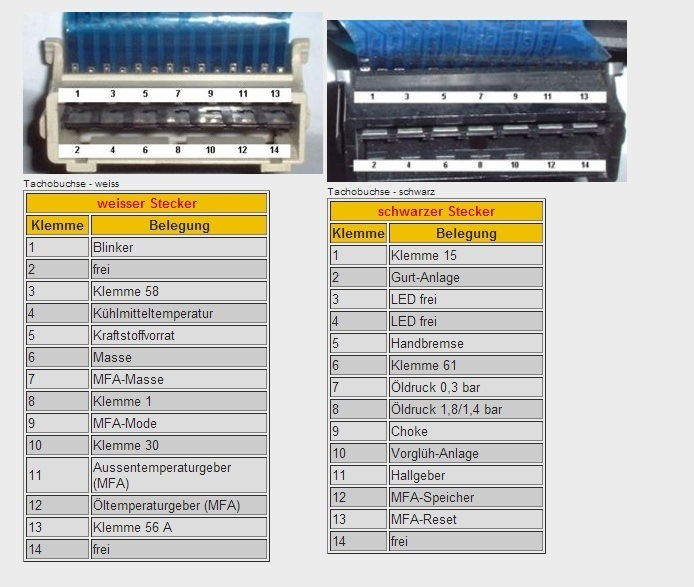
\includegraphics[width=0.72\textwidth]{digifiz_manual/image008.jpg}
    \caption{Kettős csatlakozós \ReplicaGenOne{} műszerfalak csatlakozókiosztása.}
\end{figure}

\noindent\textbf{Fehér csatlakozó}

{\scriptsize
\begin{tblr}{
    colspec={Q[l,1.4cm] X[l]},
    hlines
}
\textbf{Láb} & \textbf{Funkció} \\
1 & Irányjelző kimenet, földelve a visszajelző lámpához. \\
2 & Frei — nincs bekötve. \\
3 & 58-as kapocs, pozitív táp a háttérvilágításhoz. \\
4 & Ellenállásos hűtőfolyadék-hőmérséklet érzékelő bemenet. \\
5 & Ellenállásos üzemanyagszint-érzékelő bemenet. \\
6 & Test visszatérés. \\
7 & Kiegészítő test visszatérés. \\
8 & 1-es kapocs, motorfordulat jel (tekercs, elosztó vagy más, akár 12~V-os jel 300~V-os tüskékkel). \\
9 & MFA módvonal az MFA funkciók váltásához. \\
10 & UNR állandó pozitív táp (\ReplicaGenOneShort{} esetén nincs használatban, \ReplicaNextShort{} fő tápja). \\
11 & MFA hőmérséklet „+” vezeték a külső érzékelőhöz (\ReplicaNextShort{}). \\
12 & MFA olajhőmérséklet-érzékelő vezetéke (csak \ReplicaNextShort{}). \\
13 & KL~56a távolsági fényszóró visszajelző bemenet (+12~V aktív). \\
\end{tblr}}

\noindent\textbf{Fekete csatlakozó}

{\scriptsize
\begin{tblr}{
    colspec={Q[l,1.4cm] X[l]},
    hlines
}
\textbf{Láb} & \textbf{Funkció} \\
1 & 15-ös kapocs, gyújtásról kapcsolt +12~V. \\
2--4 & Nincs bekötve. \\
5 & Kézifék visszajelző bemenet (aktív alacsony). \\
6 & KL~61 generátor visszajelző lámpa 120~\ensuremath{\Omega}-os gerjesztő ellenállással. \\
7 & Olajnyomás kapcsoló, 0{,}3~bar. \\
8 & Olajnyomás kapcsoló, 1{,}8~bar. \\
9 & Nincs használatban. \\
10 & Izzítógyertya visszajelző bemenet (+12~V aktív, csak dízel). \\
11 & Hall-jeladó bemenet opcionális sebességérzékelőkhöz. \\
12 & MFA blokk-választó vonal. \\
13 & MFA nullázó vonal. \\
\end{tblr}}

\subsection{Egycsatlakozós műszerek}
Az egycsatlakozós műszerfalak a \autoref{fig:single-connector} ábrán látható kiosztást használják. A kábelkorbács ugyanazokat a jeleket biztosítja, mint a kétcsatlakozós változatok, de egyetlen dugóba csoportosítva.

\begin{figure}[htbp]
    \centering
    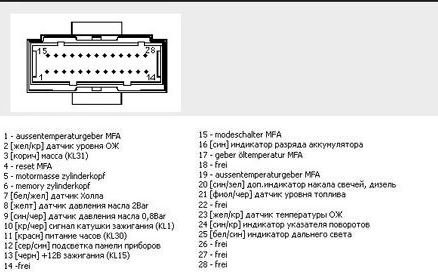
\includegraphics[width=0.65\textwidth]{digifiz_manual/image009.png}
    \caption{Az egycsatlakozós Replica műszerek kiosztása.}
    \label{fig:single-connector}
\end{figure}

\subsection{Scirocco/Passat tervezett kábelkorbács}
A tervezett Scirocco/Passat kábelkorbács két dugót használ. Funkcióikat az alábbi táblázatok foglalják össze.

\noindent\textbf{5 pólusú dugó}
{\scriptsize
\begin{tblr}{
    colspec={Q[l,2.6cm] X[l]},
    hlines
}
\textbf{Láb} & \textbf{Funkció} \\
1~(D3) & Automata váltó „D” fokozatjelző érintkezője. A hajtás visszajelzőt a földre köti, ha a választó D állásban van. \\
2~(D2) & Automata váltó második fokozatjelző érintkezője. A „2” visszajelzőt földre köti, ha a választó 2 állásban van. \\
3~(D1) & Automata váltó alacsony fokozatjelző érintkezője. Az „1” visszajelzőt földre köti, ha a választó 1 állásban van. \\
4~(SA) & Közös táp az automata fokozatkijelzőhöz (\emph{Schaltanzeige}); +12~V-ot ad a fokozatlámpáknak. \\
5~(SPERRE) & Indításgátló érintkező a választóból. Parkoló vagy üres állásban zár, így engedi a motor indítását. \\
\end{tblr}}

\noindent\textbf{14 pólusú dugó}
{\scriptsize
\begin{tblr}{
    colspec={Q[l,2.6cm] X[l]},
    hlines
}
\textbf{Láb} & \textbf{Funkció} \\
1~(KL~58) & Táp a panel háttérvilágításához. \\
2~(MASS) & Test. \\
3~(TANK) & Üzemanyagszint jeladó bemenet. \\
4~(TEMP) & Hűtőfolyadék-hőmérséklet jeladó bemenet. \\
5~(KL~1) & Fordulatszám jel (1-es kapocs). \\
6~(UHR) & Állandó +12~V az órához és a memóriához. \\
7~(FERNL) & Távolsági fényszóró visszajelző bemenet. \\
8~(reserved) & Nincs bekötve. \\
9~(OEL~1.8) & Nagynyomású olajkapcsoló, 1{,}8~bar. \\
10~(CAT~VORGL(-)) & Katalizátor-előmelegítés / dízel izzítás visszajelző bemenet (aktív alacsony). \\
11~(OEL~0.3) & Kisnyomású olajkapcsoló, 0{,}3~bar. \\
12~(KL~61) & Generátor visszajelző lámpa és gerjesztő táp. \\
13~(KL~49a) & Összekapcsolt irányjelző visszajelző táp. \\
14~(KL~15) & Gyújtásról kapcsolt +12~V táp. \\
\end{tblr}}

\subsection{Mk1 csatlakozókiosztás}
A Volkswagen Mk1 járművek az alábbi hozzárendeléseket használják:
\begin{enumerate}
    \item Világítás és tompított fényszóró táp.
    \item MASSE~31 testpont.
    \item TANK üzemanyagszint jeladó.
    \item TEMP hűtőfolyadék-hőmérséklet jeladó.
    \item KL~1 fordulatszám jel.
    \item UHR állandó +12~V.
    \item KL~56 távolsági fényszóró jel.
    \item OIL (HIGH) 1{,}8~bar nyomáskapcsoló.
    \item OIL (LOW) 0{,}3~bar nyomáskapcsoló.
    \item Dízel izzítás visszajelző.
    \item CHOKE bemenet (nincs használatban).
    \item KL~61 generátor lámpa.
    \item Irányjelző bemenet (bal/jobb kombinálva).
    \item KL~15 gyújtási táp.
\end{enumerate}
\begin{figure}[htbp]
    \centering
    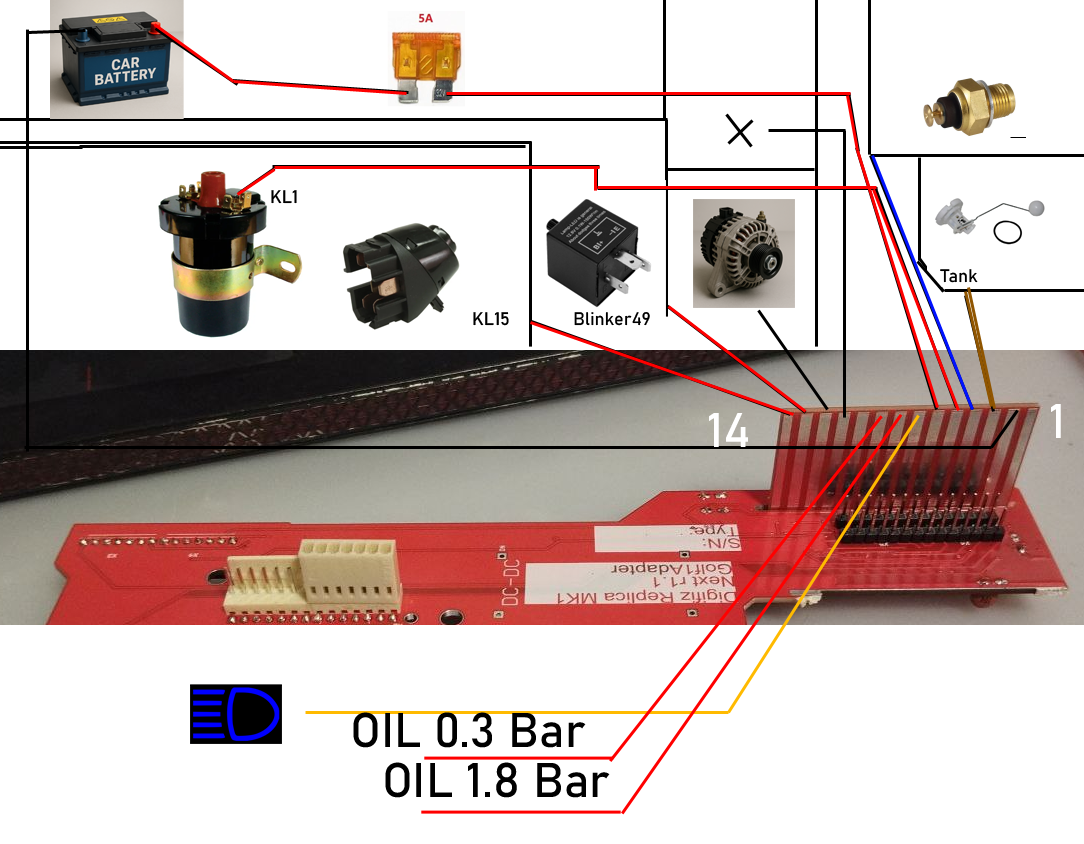
\includegraphics[width=0.75\textwidth]{digifiz_manual/image010.png}
    \caption{Kábelkorbács bekötési rajz Mk1-es beépítéshez.}
\end{figure}

\subsection{Nyomtatott áramköri lap szervizcsatlakozója}
Az áramköri lapon található harmadik csatlakozó tükrözi a műszerfal csatlakozóit; a lábak számozása \ReplicaGenOneShort{} és \ReplicaNextShort{} egységeken jobbról balra halad. Szerviz interfészt biztosít a \autoref{tab:service-connector} táblázat szerinti kiosztással.

\begin{table}[htbp]
    \centering
    \caption{A szervizcsatlakozó lábkiosztása.}
    \label{tab:service-connector}
    {\scriptsize
    \begin{tblr}{
        colspec={Q[l,1.9cm] X[l]},
        hlines,
    }
        \textbf{Pozíció} & \textbf{Funkció} \\
        1 & Visszajelző kimenet. \\
        2 & Sebességjeladó bemenet (SPM\_M). \\
        3 & Jármű test. \\
        4 & Visszajelző kimenet. \\
        5 & Bal irányjelző optocsatoló bemenet. \\
        6 & Jobb irányjelző optocsatoló bemenet. \\
        7 & Gyújtás +12~V. \\
        8 & Csak dízel specifikus bemenet. \\
        9 & Visszajelző bemenet (pozitív). \\
        10 & Alternatív fordulatszám bemenet (nincs használatban, csak \ReplicaNextShort{} esetén). \\
        11 & \ReplicaGenOneShort{}: visszajelző kimenet (általában leválasztva); \ReplicaNextShort{}: fék bemenet (aktív alacsony). \\
        12 & Fenntartva. \\
        13 & Check engine bemenet. \\
        14 & Nincs érintkező. \\
    \end{tblr}}
\end{table}

\subsection{Kiegészítő bővítőcsatlakozók}
Három kiegészítő, négytűs tüskesor található a fő panelen, hogy egyszerűsítse a kábelkorbács bővítését és a szervizelést:
\begin{itemize}
    \item \textbf{Kiegészítő analóg jelek:} dedikált bontást ad további analóg bemenetekhez egyedi érzékelők integrálásakor.
    \item \textbf{MFA tükör:} megkettőzi a szabványos \textsc{MFA} csatlakozót, így párhuzamosan ki lehet venni a fedélzeti számítógép jeleit.
    \item \textbf{Analóg duplikátumok:} ismétli az olajhőmérséklet-, külső hőmérséklet- és fék-visszajelző bemeneteket, így ezek külső adatgyűjtő vagy felügyeleti modulokra vezethetők.
\end{itemize}
Mindháromhoz \mbox{KF2510-4p} csatlakozó pár tartozik, amelyet a műszeregység készlet nem tartalmaz, így szükség esetén külön kell beszerezni.

\begin{figure}[htbp]
    \centering
    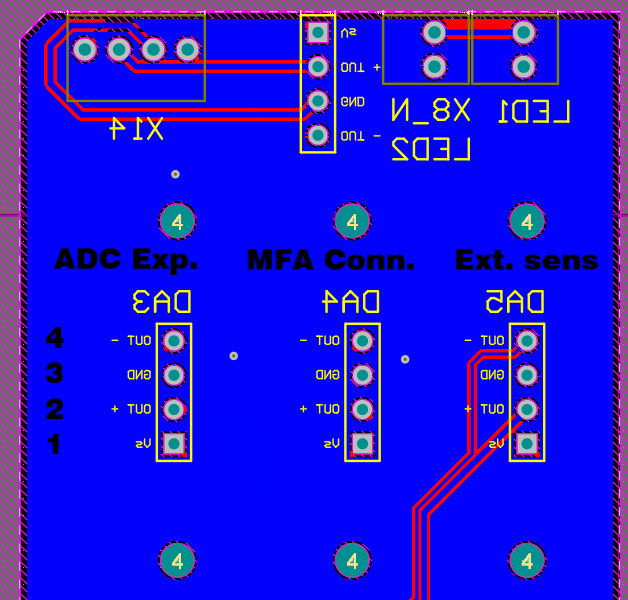
\includegraphics[width=0.6\textwidth]{digifiz_manual/ext_conn.png}
    \caption{A kiegészítő csatlakozók elhelyezkedése a fő panelen.}
\end{figure}

\begin{table}[htbp]
    \centering
    {\small
    \begin{tblr}{
        colspec={Q[l,2.3cm] Q[c,1.3cm] X[l]},
        hlines,
        row{1} = {font=\bfseries}
    }
    Csatlakozó & Láb & Funkció \\
    I. csatlakozó & 4 & Kiegészítő analóg bemenet~1 \\
    I. csatlakozó & 3 & Test (GND) \\
    I. csatlakozó & 2 & Kiegészítő analóg bemenet~2 \\
    I. csatlakozó & 1 & VCC (3V3, biztosítatlan\textbf{!!!}) \\
    II. csatlakozó & 4 & MFA nullázás \\
    II. csatlakozó & 3 & Test (GND) \\
    II. csatlakozó & 2 & MFA memória blokk \\
    II. csatlakozó & 1 & MFA mód \\
    III. csatlakozó & 4 & Olajhőmérséklet-érzékelő kimenet \\
    III. csatlakozó & 3 & Test (GND) \\
    III. csatlakozó & 2 & Külső hőmérséklet-érzékelő kimenet \\
    III. csatlakozó & 1 & Fék visszajelző \\
    \end{tblr}}
    \caption{A kiegészítő bővítőcsatlakozók lábkiosztása.}
\end{table}

\section{Beágyazott szoftver és szállítási tartalom}
A műszerfal firmware-je az alábbi címen érhető el:
\displayurl{https://github.com/Sgw32/DigifizReplica}
Kétféle kiszerelés kapható:
\begin{itemize}
    \item \textbf{\ReplicaGenOne{}:} műszeregység, külső és olajhőmérséklet-kábelkorbács, USBasp programozó és (távoli jeladó esetén) sebességérzékelő kábel.
    \item \textbf{\ReplicaNextLong{}:} műszeregység és elektronikus sebességérzékelő kábelkorbács.
\end{itemize}
